\section{Distribution of Predicted Coding Sequence Lengths}
\label{section:lengths}

To better understand and compare the distributions of CDS sequences
predicted by Braker2, GeneMark, and RefSeq, the cumulative
distribution function for the lengths of CDS sequences for each gene
finding tool are shown in Figures ~\ref{fig:cdf-lengths-1},
\ref{fig:cdf-lengths-2} and \ref{fig:cdf-lengths-3}. The $\log_{10}$
values of gene lengths were used as the abscissa for a better
visulazation of the distributions. In DC1, the curves from Braker2 and
GeneMark follow each other closely, with the only variation being
genes of short length, where Braker2's curve extends beyond that of
GeneMark, indicating that Braker2 predicts the shortest genes in all
assemblies except \textit{T. virens}. In the case of Tsth20, the
curves are nearly identical. In \textit{T. reesei}, we see
disagreement in the curves for shorter genes, with Braker2 appearing
to predict a larger fraction of shorter genes than GeneMark and
RefSeq. The right sides of the curves trend toward similar predicted
gene lengths. In \textit{T. harzianum}, RefSeq deviates from GeneMark
and Braker2, predicting more genes of short length, while Braker and
GeneMark appear to be in near-complete agreement except in the case of
very short genes. Finally, in \textit{T. virens}, we see the RefSeq
curve predicting a larger fraction of shorter genes once again,
although the deviation is not as drastic as in
\textit{T. harzianum}.From these plots, we can say that visually, gene
finding tools appear to predict different lengths of genes. We also
observe that Braker2 typically predicts the shortest genes of all
three gene finding methods.

\begin{figure}
  \centering
  \begin{subfigure}{\textwidth}
    \makebox[\textwidth]{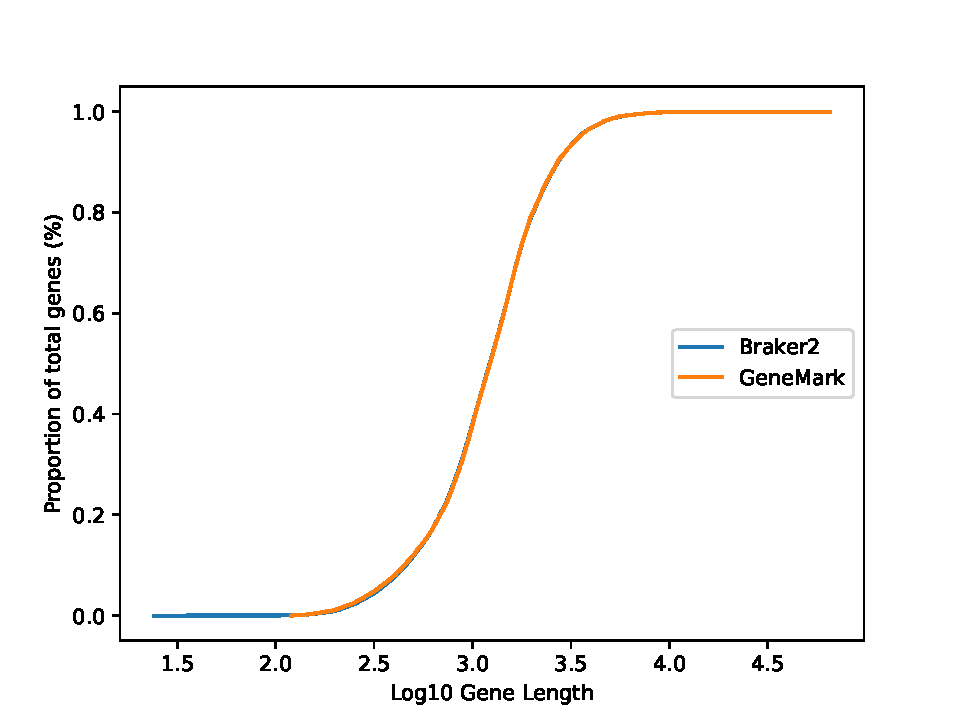
\includegraphics[width=1.1\textwidth]{figures/dc1-cdf-lengths-log.pdf}}
    \label{fig:dc1-lengths}
    \caption{DC1}
  \end{subfigure}
  \begin{subfigure}{\textwidth}
    \makebox[\textwidth]{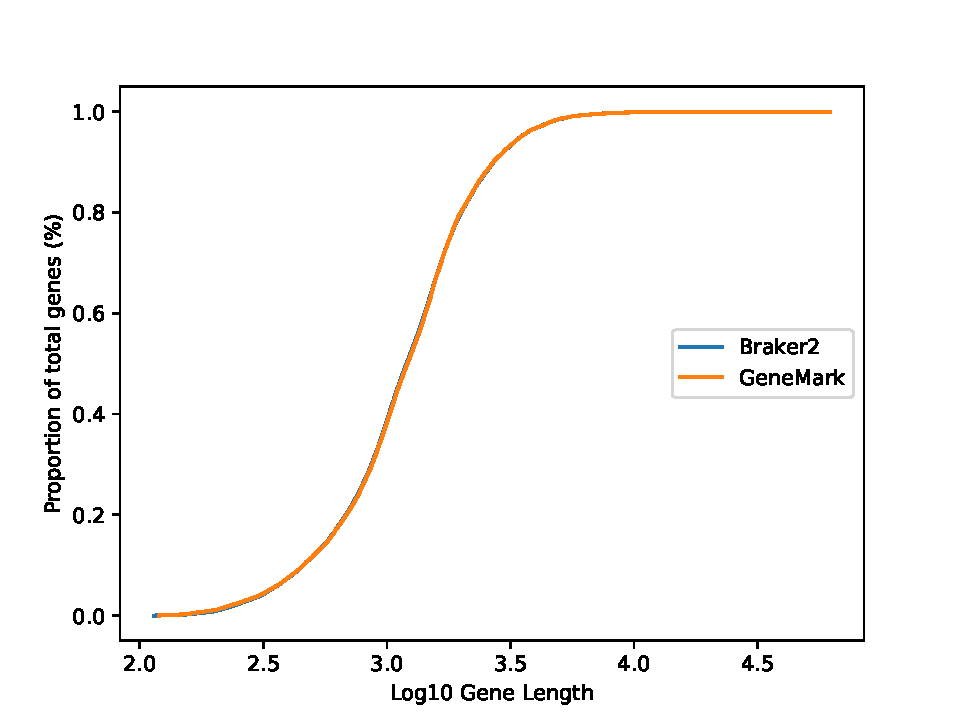
\includegraphics[width=1.1\textwidth]{figures/tsth20-cdf-lengths-log.pdf}}
    \label{fig:tsth20-lengths}
    \caption{Tsth20}
  \end{subfigure}
  \caption[CDF plots for DC1 and Tsth20]{Plots of the cumulative distribution
    function for CDS lengths produced be each gene finding tool
    applied to DC1 and Tsth20}
  \label{fig:cdf-lengths-1}
\end{figure}

\begin{figure}
  \centering
  \begin{subfigure}{\textwidth}
    \makebox[\textwidth]{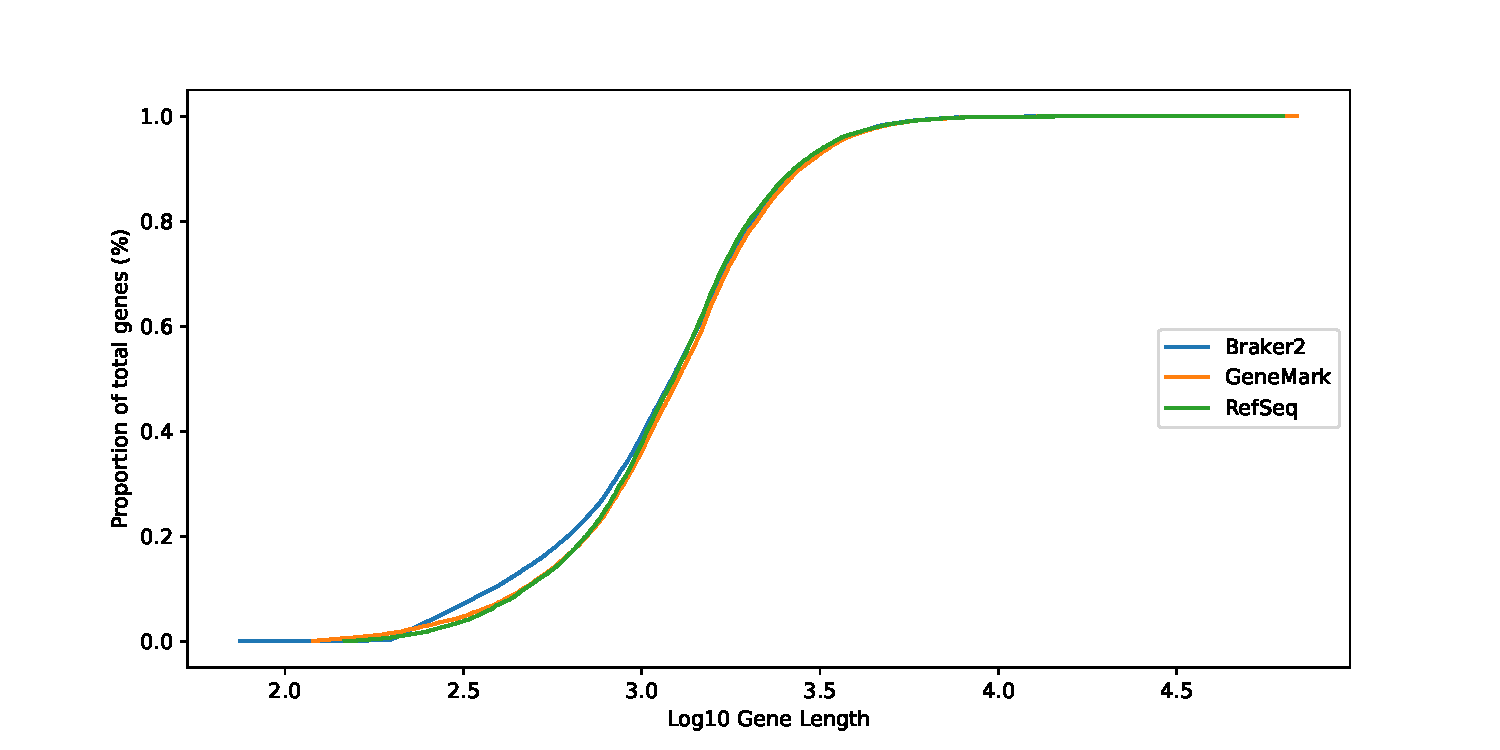
\includegraphics[width=1.1\textwidth]{figures/t-reesei-cdf-lengths-log.pdf}}
    \label{fig:treesei-lengths}
    \caption{\textit{T. reesei}}
  \end{subfigure}
  \begin{subfigure}{\textwidth}
    \makebox[\textwidth]{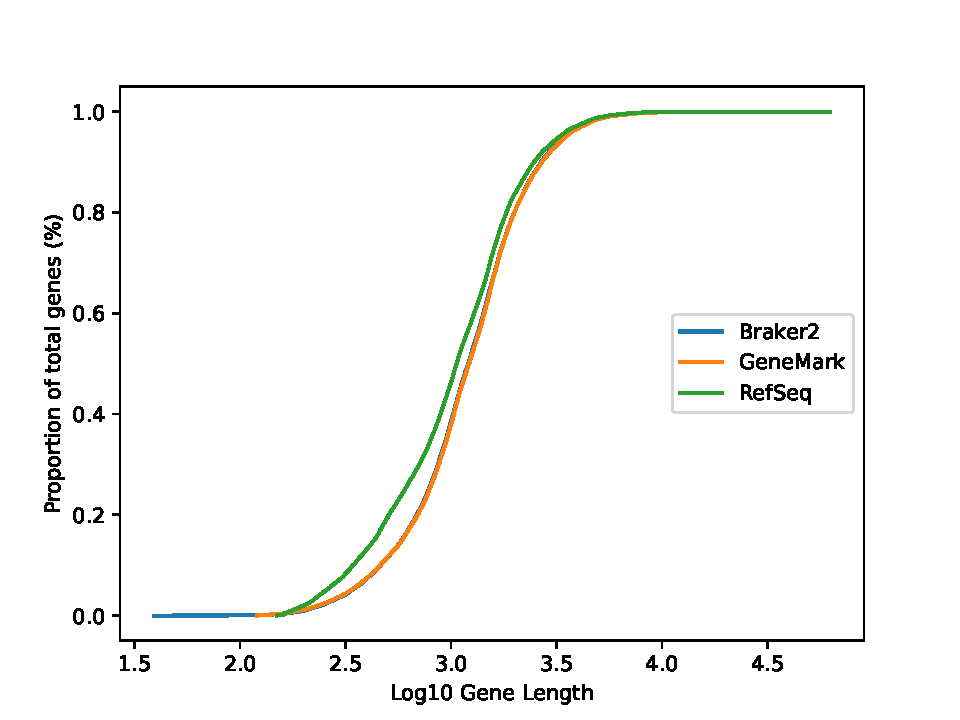
\includegraphics[width=1.1\textwidth]{figures/t-harzianum-cdf-lengths-log.pdf}}
    \label{fig:tharzianum-lengths}
    \caption{\textit{T. harzianum}}
  \end{subfigure}
  \caption[CDF plots for \textit{T. harzianum} and \textit{T. reesei}]{Plots of the cumulative distribution
    function for CDS lengths produced be each gene finding tool
    applied to \textit{T. reesei} (GCF\_000167675.1\_v2.0) and
    \textit{T. harzianum.} (GCF\_003025095.1\_Triha\_v1.0)}
  \label{fig:cdf-lengths-2}
\end{figure}

\begin{figure}
  \centering
  \begin{subfigure}{\textwidth}
    \makebox[\textwidth]{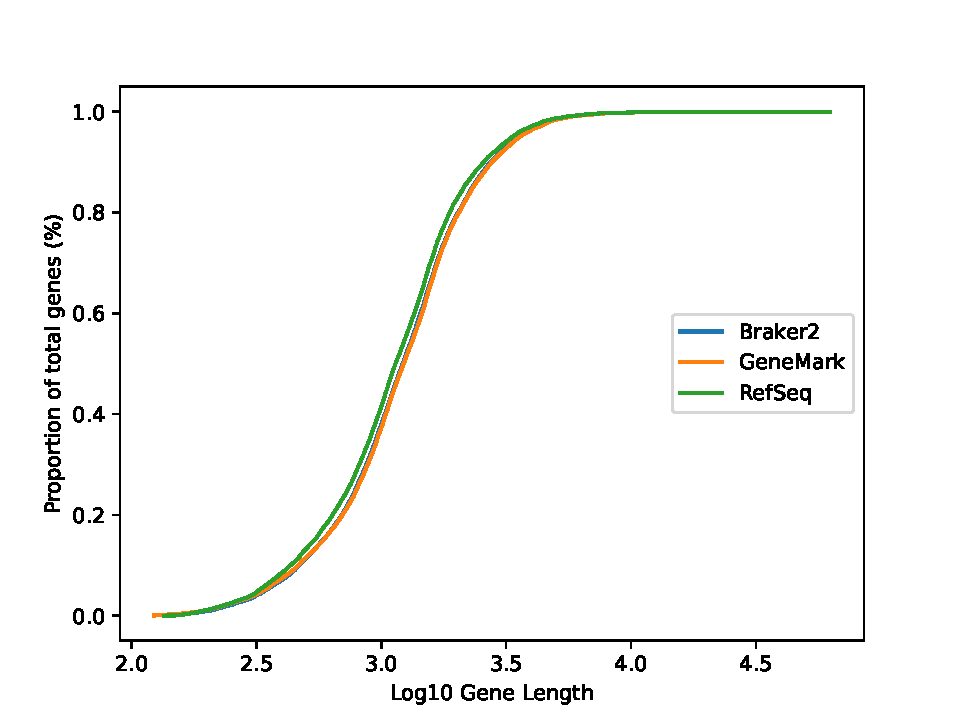
\includegraphics[width=1.1\textwidth]{figures/t-virens-cdf-lengths-log.pdf}}
    \label{fig:tvirens-lengths}
    \caption{\textit{T. virens}}
  \end{subfigure}
  \caption[CDF plots for \textit{T. virens}]{Plots of the cumulative distribution
    function for CDS lengths predicted by each gene finding tool when
    applied to \textit{T. virens} (GCF\_000170995.1\_TRIVI\_v2.0).}
  \label{fig:cdf-lengths-3}
\end{figure}

To confirm that CDF curves differ, two-sided two-sample
Kolmogorov-Smirnov\cite{ref1} tests were performed using the
$\log_{10}$ transformed gene lengths, with the null hypothesis being
that frequency of genes predicted in AT-rich and normal genomic
sequence are same. Results are presented in Table
\ref{table:ks-2s}. In the cases of DC1 and Tsth20, we see that in
agreement with Figure \ref{fig:cdf-lengths-1}, Braker2 and GeneMark do
not produce statistically different lengths of genes, which is
interesting considering that the Braker2 includes experimental
evidence for another assembly while GeneMark does not. In
\textit{T. reesei}, Braker2's predicted gene lengths are significantly
different from both RefSeq and GeneMark, which is also evident in the
CDF plots. The same cannot be said for \textit{T. harzianum} and
\textit{T. virens}, where RefSeq is significantly different from both
GeneMark and Braker2, which are not significantly different from each
other. It is also notable that RefSeq and GeneMark predict similar
gene lengths in \textit{T. reesei}, but not in \textit{T. harzianum}
and \textit{T. virens.}

\begin{table}
  \begin{center}
    \begin{tabular}{|c|c|c|c|c|c|c|}
      \hline
      Genome & Tool \#1 & Tool \#2 & \textit{P}-value  \\ \hline
      DC1 & Braker2 & GeneMark & $0.999$ \\ \hline
      Tsth20 & Braker2 & GeneMark & $0.965$ \\ \hline
      \textit{T. reesei} & Braker2 & GeneMark & $9.481*10^{-07}$ \\ \hline
      \textit{T. reesei} & GeneMark & RefSeq & $0.002$ \\ \hline
      \textit{T. reesei} & Braker2 & RefSeq & $1.340*10^{-07}$ \\ \hline
      \textit{T. harzianum} & Braker2 & GeneMark & $0.863$ \\ \hline
      \textit{T. harzianum} & GeneMark & RefSeq & $4.313*10^{-52}$ \\ \hline
      \textit{T. harzianum} & Braker2 & RefSeq & $4.674*10^{-55}$ \\ \hline
      \textit{T. virens} & Braker2 & GeneMark & $0.635$ \\ \hline
      \textit{T. virens} & GeneMark & RefSeq & $7.352*10^{-12}$ \\ \hline
      \textit{T. virens} & Braker2 & RefSeq & $1.794*10^{-09}$ \\ \hline
    \end{tabular}
  \end{center}
  \caption[Results of Kolmogorov-Smirnov tests]{Table of \textit{P}-values from two-sided two-sample
    Kolmogorov-Smirnov tests between gene finding tools.}
  \label{table:ks-2s}
\end{table}

It can clearly be stated that these gene finding tools predict
different distrbutions of gene lengths, paritcularly in
\textit{T. reesei, T. harzianum} and \textit{T. virens}. Why that may
be the case is difficult to answer without deeper invesitgation. There
is clearly an underlying difference between RefSeq and the other gene
finding tools. Braker2 and GeneMark tend to be in agreement, except in
the case of \textit{T. reesei}, for which Braker2 was specifically
trained. We observe that when Braker2 is applied to an assembly from
which the training data originated, Braker2 predicts a larger fraction
of shorter genes. Conversly, we observe that when Braker2 is trained
with experimental evidence and applied to a \textit{Trichoderma}
assembly from which the training data did not originate, the
distributions of predicted genes lengths do not significantly differ
from the \textit{ab initio} gene finder GeneMark.
